\documentclass[12pt]{exam}
\usepackage{amsthm}
\usepackage{libertine}
\usepackage[utf8]{inputenc}
\usepackage[margin=1in]{geometry}
\usepackage{amsmath,amssymb}
\usepackage{multicol}
\usepackage[shortlabels]{enumitem}
\usepackage{siunitx}
\usepackage{booktabs}
\usepackage{graphicx}
\usepackage{pgfplots}
\usepackage{listings}
\usepackage{tikz}



\pgfplotsset{width=10cm,compat=1.9}
\usepgfplotslibrary{external}
%\tikzexternalize

\newcommand{\class}{Math 101-002} % This is the name of the course 
\newcommand{\examnum}{Exam 3} % This is the name of the assignment
\newcommand{\examdate}{April 17} % This is the due date





\begin{document}
\pagestyle{plain}
\thispagestyle{empty}

\noindent
\textbf{\class}\\
\textbf{\examnum}, \textbf{\examdate} \\

% Name \hfill CSU ID \# \hspace{2.25in}

%\vspace{10 pt}

\setlength{\tabcolsep}{3.5cm} % Default value: 6pt
\renewcommand{\arraystretch}{1.5}
\setlength\extrarowheight{1cm}
\begin{tabular}{ |c|c| } 
 \hline
 Name   & CSU ID \#  \\ 
 \hline
\end{tabular}
% ---
\vspace{10pt}

Be sure to read each question fully and carefully. Multiple choice answer bubbles must be fully filled in.  There is space to the right of each multiple choice question to show work, if your work is correct you can get points even with an incorrect multiple choice answer.  


\iffalse

    \foreach \s in {1,...,5}{
          \choice $P_\s$ has no power 
     }%;
\fi


\begin{enumerate} 

\item For questions \ref{firstQnSec1} through \ref{lastQnSec1} consider the following information about a weighted graph $G$ with vertices $A$ through $E$:\par
\begin{figure}[h]
    \centering
    \includegraphics{tableQ1.pdf}
\end{figure}

\begin{enumerate}
    \item \label{firstQnSec1} Based on the information presented in the tableau, fill in the edges of the graph $G$ with their corresponding weights: (4 points)
    \begin{figure}[h!]
        \centering
       

        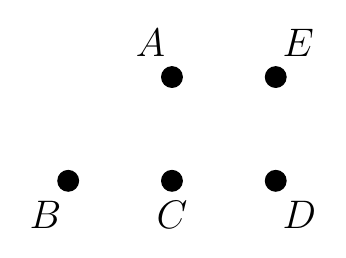
\begin{tikzpicture}[x=0.75pt,y=0.75pt,yscale=-1,xscale=1]
            %uncomment if require: \path (0,300); %set diagram left start at 0, and has height of 300
            
            %Shape: Ellipse [id:dp34886352038339286] 
            \draw  [fill={rgb, 255:red, 0; green, 0; blue, 0 }  ,fill opacity=1 ] (100,105) .. controls (100,102.24) and (102.24,100) .. (105,100) .. controls (107.76,100) and (110,102.24) .. (110,105) .. controls (110,107.76) and (107.76,110) .. (105,110) .. controls (102.24,110) and (100,107.76) .. (100,105) -- cycle ;
            %Shape: Ellipse [id:dp5240816285463924] 
            \draw  [fill={rgb, 255:red, 0; green, 0; blue, 0 }  ,fill opacity=1 ] (150,105) .. controls (150,102.24) and (152.24,100) .. (155,100) .. controls (157.76,100) and (160,102.24) .. (160,105) .. controls (160,107.76) and (157.76,110) .. (155,110) .. controls (152.24,110) and (150,107.76) .. (150,105) -- cycle ;
            %Shape: Ellipse [id:dp7816117134537868] 
            \draw  [fill={rgb, 255:red, 0; green, 0; blue, 0 }  ,fill opacity=1 ] (100,155) .. controls (100,152.24) and (102.24,150) .. (105,150) .. controls (107.76,150) and (110,152.24) .. (110,155) .. controls (110,157.76) and (107.76,160) .. (105,160) .. controls (102.24,160) and (100,157.76) .. (100,155) -- cycle ;
            %Shape: Ellipse [id:dp24376001324989727] 
            \draw  [fill={rgb, 255:red, 0; green, 0; blue, 0 }  ,fill opacity=1 ] (150,155) .. controls (150,152.24) and (152.24,150) .. (155,150) .. controls (157.76,150) and (160,152.24) .. (160,155) .. controls (160,157.76) and (157.76,160) .. (155,160) .. controls (152.24,160) and (150,157.76) .. (150,155) -- cycle ;
            %Shape: Ellipse [id:dp7315021942502884] 
            \draw  [fill={rgb, 255:red, 0; green, 0; blue, 0 }  ,fill opacity=1 ] (50,155) .. controls (50,152.24) and (52.24,150) .. (55,150) .. controls (57.76,150) and (60,152.24) .. (60,155) .. controls (60,157.76) and (57.76,160) .. (55,160) .. controls (52.24,160) and (50,157.76) .. (50,155) -- cycle ;
            
            % Text Node
            \draw (103,96.6) node [anchor=south east] [inner sep=0.75pt]  [font=\Large]  {$A$};
            % Text Node
            \draw (157,96.6) node [anchor=south west] [inner sep=0.75pt]  [font=\Large]  {$E$};
            % Text Node
            \draw (53,163.4) node [anchor=north east] [inner sep=0.75pt]  [font=\Large]  {$B$};
            % Text Node
            \draw (105,163.4) node [anchor=north] [inner sep=0.75pt]  [font=\Large]  {$C$};
            % Text Node
            \draw (157,163.4) node [anchor=north west][inner sep=0.75pt]  [font=\Large]  {$D$};
            
            
            \end{tikzpicture}
            
    
    
    
    
    \end{figure}
    \vfill
    \item What is the degree of separation between the vertices $B$ and $D$? (2 points)
    \begin{checkboxes}
        \foreach \s in {1,...,4}{
            \choice $\s$ 
       }%;
    \end{checkboxes}
    \vfill
    \item What is the degree of separation between the vertices $B$ and $E$? (2 points)
    \begin{checkboxes}
        \foreach \s in {1,...,4}{
            \choice $\s$ 
       }%;
    \end{checkboxes}
    \vfill
    \item The diameter of the graph $G$ is: (2 points)
    \vspace{0.5em}
    $$\operatorname{diam}(G)=\underline{\phantom{ans}}.$$
    \vfill
    \item The redundancy of the graph $G$ is: (2 points)
    \vspace{0.5em}
    $$\operatorname{red}(G)=\underline{\phantom{ans}}.$$

    \item Between the following, mark the option which is not a spanning tree of $G$: (2 points)
    \begin{checkboxes}
        \choice $AB,BC,CD,AE$
        \choice $AB,AD,AE,DE$
        \choice $AC,AD,BC,DE$
        \choice $AD,AE,BC,CD$
    \end{checkboxes}


    \item \label{lastQnSec1} Write down the weight of the minimal spanning tree produced by Kruskal's algorithm: (2 points)
    \vspace{0.5em}
    $$\text{weight}(MST)=\underline{\phantom{ans}}.$$

    Help yourself by drawing the tree in question in what follows:
    \vspace{0.5cm}
    \begin{figure}[h!]
        \centering
       

        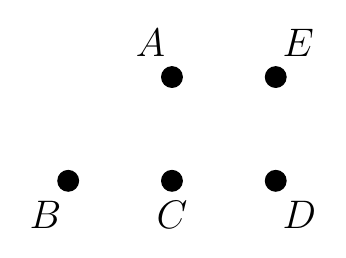
\begin{tikzpicture}[x=0.75pt,y=0.75pt,yscale=-1,xscale=1]
            %uncomment if require: \path (0,300); %set diagram left start at 0, and has height of 300
            
            %Shape: Ellipse [id:dp34886352038339286] 
            \draw  [fill={rgb, 255:red, 0; green, 0; blue, 0 }  ,fill opacity=1 ] (100,105) .. controls (100,102.24) and (102.24,100) .. (105,100) .. controls (107.76,100) and (110,102.24) .. (110,105) .. controls (110,107.76) and (107.76,110) .. (105,110) .. controls (102.24,110) and (100,107.76) .. (100,105) -- cycle ;
            %Shape: Ellipse [id:dp5240816285463924] 
            \draw  [fill={rgb, 255:red, 0; green, 0; blue, 0 }  ,fill opacity=1 ] (150,105) .. controls (150,102.24) and (152.24,100) .. (155,100) .. controls (157.76,100) and (160,102.24) .. (160,105) .. controls (160,107.76) and (157.76,110) .. (155,110) .. controls (152.24,110) and (150,107.76) .. (150,105) -- cycle ;
            %Shape: Ellipse [id:dp7816117134537868] 
            \draw  [fill={rgb, 255:red, 0; green, 0; blue, 0 }  ,fill opacity=1 ] (100,155) .. controls (100,152.24) and (102.24,150) .. (105,150) .. controls (107.76,150) and (110,152.24) .. (110,155) .. controls (110,157.76) and (107.76,160) .. (105,160) .. controls (102.24,160) and (100,157.76) .. (100,155) -- cycle ;
            %Shape: Ellipse [id:dp24376001324989727] 
            \draw  [fill={rgb, 255:red, 0; green, 0; blue, 0 }  ,fill opacity=1 ] (150,155) .. controls (150,152.24) and (152.24,150) .. (155,150) .. controls (157.76,150) and (160,152.24) .. (160,155) .. controls (160,157.76) and (157.76,160) .. (155,160) .. controls (152.24,160) and (150,157.76) .. (150,155) -- cycle ;
            %Shape: Ellipse [id:dp7315021942502884] 
            \draw  [fill={rgb, 255:red, 0; green, 0; blue, 0 }  ,fill opacity=1 ] (50,155) .. controls (50,152.24) and (52.24,150) .. (55,150) .. controls (57.76,150) and (60,152.24) .. (60,155) .. controls (60,157.76) and (57.76,160) .. (55,160) .. controls (52.24,160) and (50,157.76) .. (50,155) -- cycle ;
            
            % Text Node
            \draw (103,96.6) node [anchor=south east] [inner sep=0.75pt]  [font=\Large]  {$A$};
            % Text Node
            \draw (157,96.6) node [anchor=south west] [inner sep=0.75pt]  [font=\Large]  {$E$};
            % Text Node
            \draw (53,163.4) node [anchor=north east] [inner sep=0.75pt]  [font=\Large]  {$B$};
            % Text Node
            \draw (105,163.4) node [anchor=north] [inner sep=0.75pt]  [font=\Large]  {$C$};
            % Text Node
            \draw (157,163.4) node [anchor=north west][inner sep=0.75pt]  [font=\Large]  {$D$};
            
            
            \end{tikzpicture}
            
    
    
    
    
    \end{figure}
\end{enumerate}
    \vfill
    \newpage
    \item For questions \ref{firstQnSec2} through \ref{lastQnSec2} consider the following graph:\par
\begin{figure}[h]
    \centering
    \includegraphics[width=0.5\textwidth]{graph1.png}
\end{figure}
\begin{enumerate}
    \item \label{firstQnSec2}Between the following options, which is a spanning tree that makes $D$ and $K$ have degree of separation $4$? (2 points)
    \begin{checkboxes}
        \choice $AB,AC,BD,BE,CF,DG,FI,GJ,HK,IK$
        \choice $AC,BD,BE,CE,CF,DG,EI,GJ,HJ,IK$
        \choice $AC,BE,CF,DH,EI,FI,GJ,HJ,HK,IK$
        \choice $AB,CE,CF,DG,EH,FI,GJ,HJ,HK,IK$
    \end{checkboxes}
    Help yourself with three other copies of the graph:
    \begin{center}
    \includegraphics[width=0.25\textwidth]{graph1.png}
    \includegraphics[width=0.25\textwidth]{graph1.png}
    \includegraphics[width=0.25\textwidth]{graph1.png}
    \end{center}
    \item Write down the degree of separation of the vertices $F$ and $G$: (2 points)
    $$d(F,G)=\underline{\phantom{ans}}$$
    \item Write down the redundancy of the graph $G$: (2 points)
    $$\text{red}(G)=\underline{\phantom{ans}}$$
    \item \label{lastQnSec2} Between the following pairs of vertices, only pair has a different degree of separation. Find it: (2 points)
    \begin{checkboxes}
        \choice $A$ and $H$
        \choice $B$ and $F$
        \choice $I$ and $G$
        \choice $C$ and $J$
    \end{checkboxes}
    \vfill
\end{enumerate}
    \newpage
\item For questions \ref{firstQnSec3} through \ref{lastQnSec3} consider the following tableau with information on a project with six tasks $A$ through $E$:\par
    \begin{figure}[h]
        \centering
        \includegraphics[width=0.4\textwidth]{tableQ3.pdf}
    \end{figure}
\begin{enumerate}
    \item \label{firstQnSec3} Fill in the project digraph with the processing times and precedence relations: (4 points)
    \begin{figure}[h]
        \centering
        \includegraphics[width=0.75\textwidth]{ProjDigraph1.png}
    \end{figure}
    \vfill 
\item Apply the backflow algorithm to find the critical time of each task: (4 points)
\begin{figure}[h]
    \centering
    \includegraphics[width=0.75\textwidth]{ProjDigraph2.png}
\end{figure}
\vfill 
\newpage
\item What is the critical time for this project? (2 points)
$$\text{Project Critical Time}=\underline{\phantom{ans}}.$$
\item Write down a priority list of tasks based on the critical path algorithm: (2 points)
$$\text{Project List}=\left\lbrace\underline{\phantom{ans}},\underline{\phantom{ans}},\underline{\phantom{ans}},\underline{\phantom{ans}},\underline{\phantom{ans}},\underline{\phantom{ans}}\right\rbrace.$$\\
\item \label{lastQnSec3} Using the critical path algorithm create a schedule for two workers: (4 points)
\begin{figure}[h!]
    \centering
    \includegraphics[width=0.6\textwidth]{ScheduleQ3.png}
\end{figure}
\vfill
\end{enumerate}
\newpage
\item Short answer:
\begin{enumerate}
    \item Suppose a connected graph has $16$ vertices and $64$ edges. How many edges will any of its spanning trees have? (4 points)
    \vspace{3cm}
    \item We defined a \emph{tree} as a connected graph with no cycles. Mention any of the three properties equivalent to being a tree. (4 points)
    \vspace{3cm}
    \item Consider your family tree as a graph where the relation is $A$ is connected to $B$ if $A$ is $B$'s kid. Assume you have a nephew, what is the degree of separation between yourself and your nephew? (4 points)
    \vspace{3cm}
\end{enumerate}


\item In the following space draw the requested graphs:
\begin{enumerate}
    \item A directed graph with a directed cycle. (4 points)
    \vspace{3.5cm}
    \item A directed graph without a directed cycle. (4 points)
    \vfill
\end{enumerate}

\iffalse
Sol:
\begin{enumerate}
    \item A walk starts and ends at different places whereas a circuit begins and ends at the same place.
    \item Eulerian means that edges are the object of interest to traverse, while Hamiltonian means that the vertices are the traversed ones.
    \item Any path graph.
    \item A path graph with any pair of middle vertices connected.
    \item Two triangles joined at a vertex, say a ribbon.
    \item The ribbon graph again.
    \item A cycle with more than four vertices with any two non-adjacent vertices connected.
\end{enumerate}
\fi
\newpage
\item (25 points) Realistically, when you're traveling in your local city, you're very likely to know your neighborhood and your route to your worksite. It is also likely that you know the places you frequent often such as the supermarket and houses of friends you visit often.\par
In this hypothetical scenario, you're driving to a concert this weekend and need to pick up several friends along the way. Some friends live close to you, while others are farther away in areas you're not familiar with. You also don't know the concert venue very well.\par
For this scenario, assume you have a physical map of the city and the addresses of your friends, but no access to GPS or navigation apps.\par
In the following space address the following prompts and discuss thoroughly and explain your reasonings:
\begin{itemize}
    \item Do you think that this situation is better modeled through an Eulerian or Hamiltonian approach? Are you trying to make a walk or a circuit? 
    \item Since some friends live nearby and others farther away, where you're not familiar, would that influence your choice of algorithm to pick up? Why?
    \item Could a mix of algorithms make for a better route?
    \item If you're running late or some friends aren't ready yet, how does that change your approach? Would it affect your choice of algorithm or the order in which you pick people up? Why or why not?
\end{itemize}

Sol:
\begin{itemize}
    \item 8 pts clearly explains whether the situation is more Hamilton or Euler and adds evidence to support reasonings.
    \item 6 pts discusses how friends locations affects choice of approach
    \item 6 pts thoroughly considers whether a hybrid strategy would be beneficial.
    \item 5 pts similarly discusses how a time constraint could affect the choice.
\end{itemize}

\end{enumerate}
\end{document}

